\documentclass[11pt]{article}
\usepackage[margin=1in]{geometry}
\usepackage{amsmath,amssymb}
\usepackage{booktabs}
\usepackage{graphicx}
\usepackage{subcaption}
\usepackage[hidelinks]{hyperref}

\title{Learning-Augmented Densest At-Most-$k$ Subgraph\\on Twitch Ego-Nets}
\author{}
\date{October 2, 2026}

\begin{document}
\maketitle

\section{Setup}

\paragraph{Problem.} Given $G=(V,E)$ and $k$, find $H \subseteq V$ with $|H|\le k$
maximizing $d(H) = e(H)/|H|$. We use $k=15$.

\paragraph{Data.} 500 Twitch ego-nets ($30 \le n \le 52$, mean $n=40.4$, mean $m=136.9$).
Edges are treated as undirected and deduplicated; the source edge list
lists about two-thirds of edges in both directions.

\paragraph{Ground truth.} Exact optima $H^\star$ are computed by an ILP
(JuMP + HiGHS) inside Dinkelbach's method: given the current best set with $e$ edges on
$s$ vertices, solve
\[
\max\; s\textstyle\sum_{uv} y_{uv} - e \sum_v x_v
\quad\text{s.t.}\quad y_{uv}\le x_u,\; y_{uv}\le x_v,\; 1\le \textstyle\sum_v x_v \le k,\; x\in\{0,1\}^V,
\]
with valid degree cuts $\sum_{u\in N(v)} y_{uv} \le \min\{\sum_w x_w - x_v,\,(k-1)x_v\}$.
A positive optimum gives a strictly denser set; an optimum of $0$ certifies optimality.
All 500 instances are solved to proven optimality; $|H^\star|$ ranges from 5 to 15.

\paragraph{Predictor.} A random forest (100 trees) outputs $p(v)\approx\Pr[v\in H^\star]$
from per-vertex features: degree, average neighbor degree, $n$, core number, and local
clustering coefficient. The predicted set is $S=\{v : p(v)\ge 1/2\}$.
We use 5-fold cross-validation over graphs, so each graph is evaluated by a model that
never saw it.

\paragraph{Learning-augmented DamkS.} Given $S$ and $\varepsilon$:
\begin{enumerate}
  \item $r \leftarrow \min\{\lceil \tfrac{\varepsilon}{1-\varepsilon}|S|\rceil,\, |V\setminus S|\}$;
  \item $U \leftarrow$ the $r$ vertices of $V\setminus S$ with the largest $e(v,S)$;
  \item $T \leftarrow S\cup U$; while $|T|>k$, remove a minimum-degree vertex of $G[T]$;
  \item return $T$.
\end{enumerate}
$\varepsilon$ is estimated per fold as the mean of $|S\,\triangle\,H^\star|/|H^\star|$ on a
held-out 20\% calibration split of the training graphs ($\hat\varepsilon \in [0.44, 0.48]$).

\paragraph{Baseline.} \emph{Predictor only} returns $S$ itself. Note that $S$ is
\emph{infeasible} ($|S|>k$) on 205 of 500 graphs. We also report the top-$k$ vertices by $p(v)$,
which is always feasible.

\section{Results}

\paragraph{Predictor quality.} Mean $|S\,\triangle\,H^\star|/|H^\star| = 0.48$, mean
$\sum_v|p(v)-\mathbf{1}[v\in H^\star]|/|H^\star| = 0.58$; mean $|S|=13.3$ vs.\ mean $|H^\star|=13.8$.
This is a weak predictor, well outside the small-$\varepsilon$ regime of the theory.

\paragraph{Solution quality.} Table~\ref{tab:quality} reports $d(\text{output})/d(H^\star)$.

\begin{table}[h]
\centering
\begin{tabular}{lccccc}
\toprule
Method & Mean & Median & Min & $\ge 0.95$ & Optimal \\
\midrule
\textbf{Learning-augmented DamkS} ($\hat\varepsilon$) & \textbf{0.937} & \textbf{0.996} & 0.250 & \textbf{74.6\%} & \textbf{48.4\%} \\
Predictor only ($S$, all graphs)          & 0.817 & 0.907 & 0.000 & 35.0\% & 18.2\% \\
\quad graphs with $|S|\le k$ only ($n=295$) & 0.705 & 0.810 & 0.000 & 14.2\% & 2.7\% \\
\quad infeasible outputs scored as 0      & 0.416 & 0.420 & 0.000 & 8.4\% & 1.6\% \\
Top-$k$ by $p(v)$                         & 0.894 & 0.913 & 0.532 & 27.4\% & 6.6\% \\
\bottomrule
\end{tabular}
\caption{Approximation ratio over 500 graphs ($k=15$). The ``all graphs'' predictor-only row
counts infeasible outputs at face value and therefore overstates that baseline.}
\label{tab:quality}
\end{table}

Per graph, learning-augmented DamkS beats predictor only on 387 graphs, ties on 7, and
loses on 106; in 86 of those losses the predictor's $S$ was infeasible. The mean ratio
gain is $+0.120$.

\paragraph{Running time.} Table~\ref{tab:time} compares the cost of obtaining a solution with
the exact ILP against learning-augmented DamkS. Both are run single-threaded on the same
machine (AMD Ryzen 9 9900X, Julia 1.11, HiGHS with 1 thread). The learning-augmented time is
end-to-end: feature computation, forest inference, and the algorithm. The one-time cost of
training the forest is excluded.

\begin{table}[h]
\centering
\begin{tabular}{lrrrrr}
\toprule
 & Mean & Median & 90th pct & Max & Total \\
\midrule
Exact ILP                                 & 213 ms   & 17.9 ms  & 617 ms   & 4480 ms & 107 s \\
Learning-aug.\ DamkS (end-to-end) & 0.289 ms & 0.290 ms & 0.414 ms & 1.06 ms & 0.144 s \\
\quad algorithm only & 0.009 ms & 0.009 ms & 0.016 ms & 0.027 ms & 0.005 s \\
\bottomrule
\end{tabular}
\caption{Time per graph. Per-graph speed-up of learning-augmented DamkS over the ILP: median
$74\times$, minimum $19.5\times$; ratio of total times $738\times$.}
\label{tab:time}
\end{table}

\begin{table}[h]
\centering
\begin{tabular}{lrrrrr}
\toprule
$n$ & Graphs & Mean $m$ & ILP mean / median & Learning-aug.\ mean & Learning-aug.\ ratio \\
\midrule
30--39 & 242 & 105 & 82 ms / 10 ms  & 0.24 ms & 0.940 \\
40--46 & 135 & 148 & 262 ms / 30 ms & 0.33 ms & 0.923 \\
47--52 & 123 & 187 & 417 ms / 64 ms & 0.34 ms & 0.948 \\
\bottomrule
\end{tabular}
\caption{By graph size. ILP time grows quickly with $n$ and has a heavy tail;
learning-augmented DamkS stays essentially flat with no loss in quality.}
\label{tab:size}
\end{table}

\begin{figure}[h]
\centering
\begin{subfigure}{0.48\textwidth}
  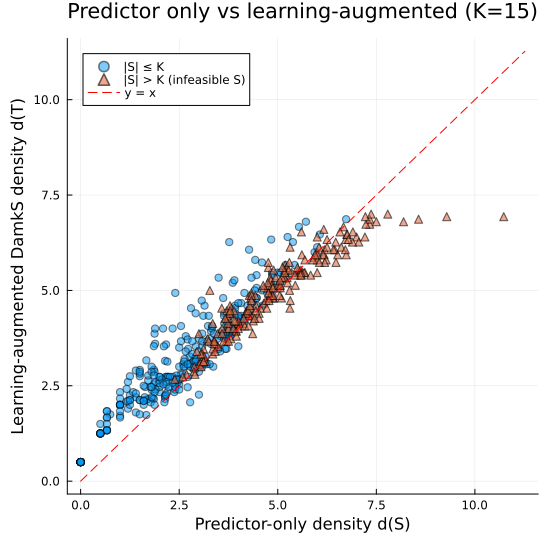
\includegraphics[width=\linewidth]{../damks_pred_predictor_vs_algorithm.png}
  \caption{Per-graph density: predictor only vs.\ learning-augmented DamkS.
  Triangles mark graphs where $S$ is infeasible.}
\end{subfigure}\hfill
\begin{subfigure}{0.48\textwidth}
  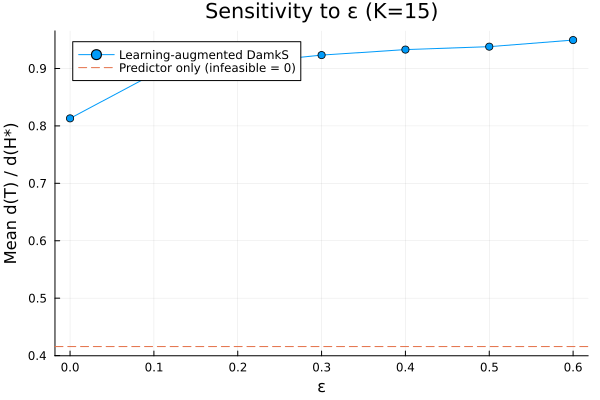
\includegraphics[width=\linewidth]{../damks_pred_eps_sweep.png}
  \caption{Mean ratio vs.\ fixed $\varepsilon$. $\varepsilon=0$ only trims $S$ to $k$.}
\end{subfigure}
\caption{Learning-augmented DamkS vs.\ predictor only.}
\label{fig:main}
\end{figure}

\paragraph{Sensitivity to $\varepsilon$.} With fixed $\varepsilon$, the mean ratio rises
monotonically: 0.813 ($\varepsilon=0$), 0.891 (0.1), 0.908 (0.2), 0.923 (0.3), 0.933 (0.4),
0.938 (0.5), 0.950 (0.6). Adding the $U$ vertices before trimming is what drives the
improvement: trimming $S$ alone ($\varepsilon=0$) gives 0.813, about the same as predictor only
at face value (0.817), although it is always feasible.

\section{Takeaways}
\begin{itemize}
  \item Even with a weak predictor ($\varepsilon\approx 0.48$), learning-augmented DamkS
  attains a mean ratio of 0.937 (median 0.996) and is exactly optimal on 48\% of graphs,
  versus 0.817 / 18\% for the predictor's set. Its output is always feasible, whereas the
  predictor's set violates $|S|\le k$ on 41\% of graphs.
  \item It is about $74\times$ faster than the exact ILP per graph (median) and $738\times$
  faster in total, and its cost does not grow with the ILP's heavy tail.
  \item The weakest point is the worst case (min ratio 0.25), caused by poor predictions on a
  few graphs; a stronger predictor should tighten this.
\end{itemize}

\end{document}
